\section{AU --- Evidencia Aut\'onoma: Selecci\'on de Caracter\'isticas Avanzada}

\subsection{Variable Objetivo}

\textbf{Target:} \texttt{alerta\_temperatura} = 1 si temperatura $>$ 35\textcelsius{}

Owens (1971) y Seeley (1985) documentan que por encima de 35\textcelsius{} las abejas de
ventilaci\'on (\textit{fanners}) se activan masivamente, lo que se manifiesta en un
incremento del nivel sonoro, descenso de humedad interior y potencial p\'erdida de peso
por enjambre. Distribuci\'on: 8\,364 negativos (97.6\%) y 209 positivos (2.4\%).

\subsection{M\'etodo 1 --- Correlaci\'on de Pearson}

La correlaci\'on de Pearson mide la relaci\'on lineal entre cada variable num\'erica y el
target. Umbral de corte: $|r| \geq 0.02$. Ninguna feature fue descartada por este
m\'etodo --- todas presentan alguna relaci\'on lineal con \texttt{alerta\_temperatura}.

\begin{figure}[h!]
  \centering
  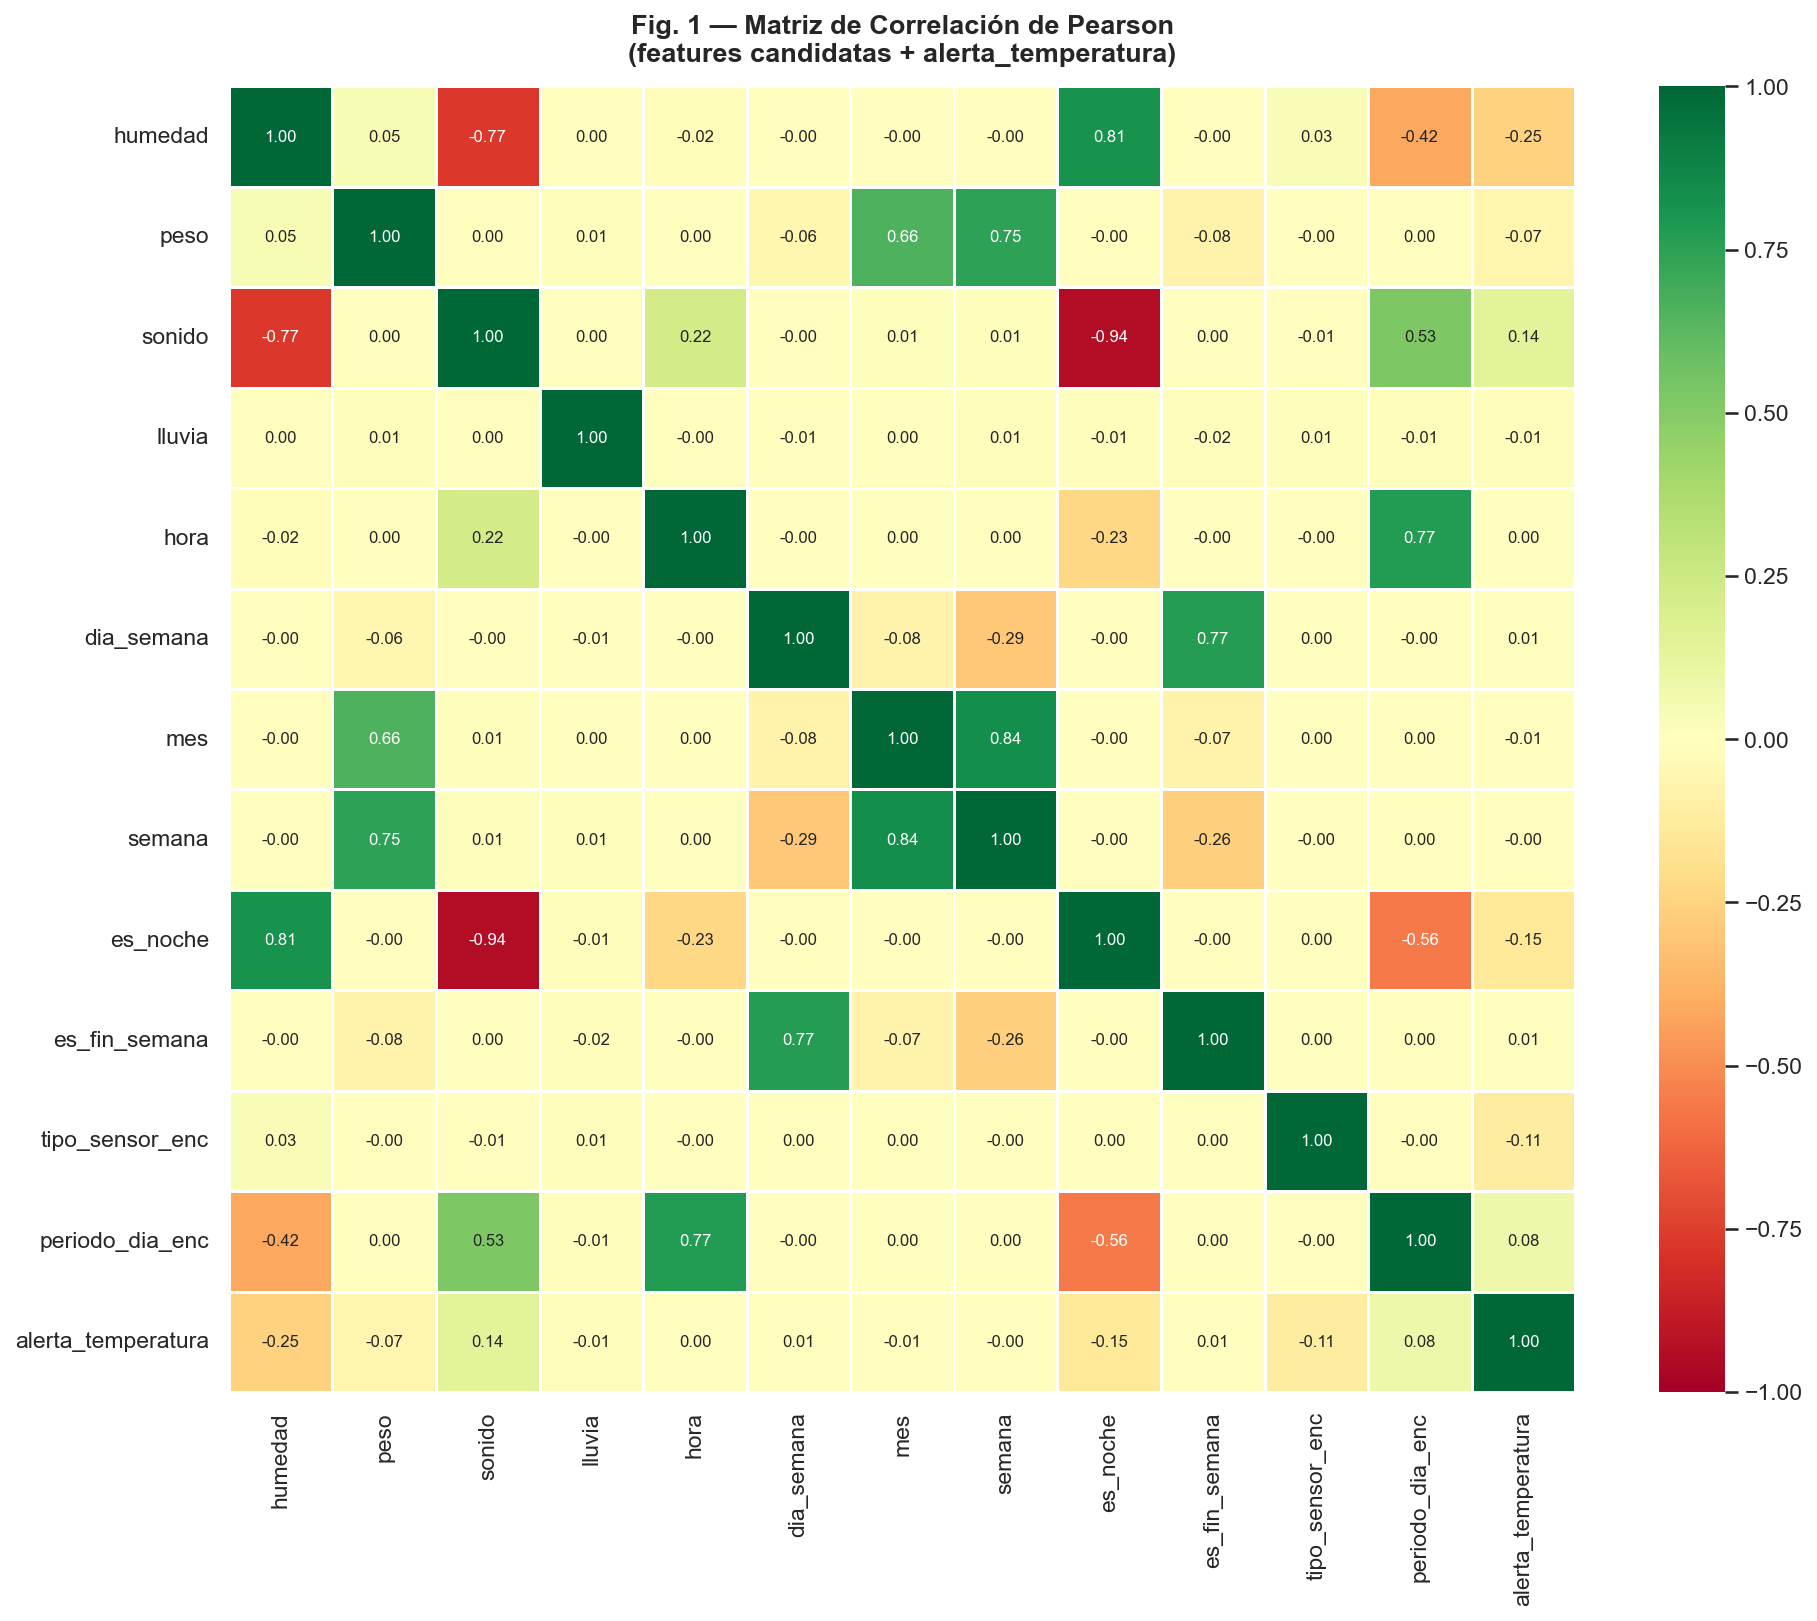
\includegraphics[width=\textwidth]{figures/fig1_heatmap_correlacion.png}
  \caption{Matriz completa de correlaci\'on de Pearson (features candidatas + target)}
\end{figure}

\begin{figure}[h!]
  \centering
  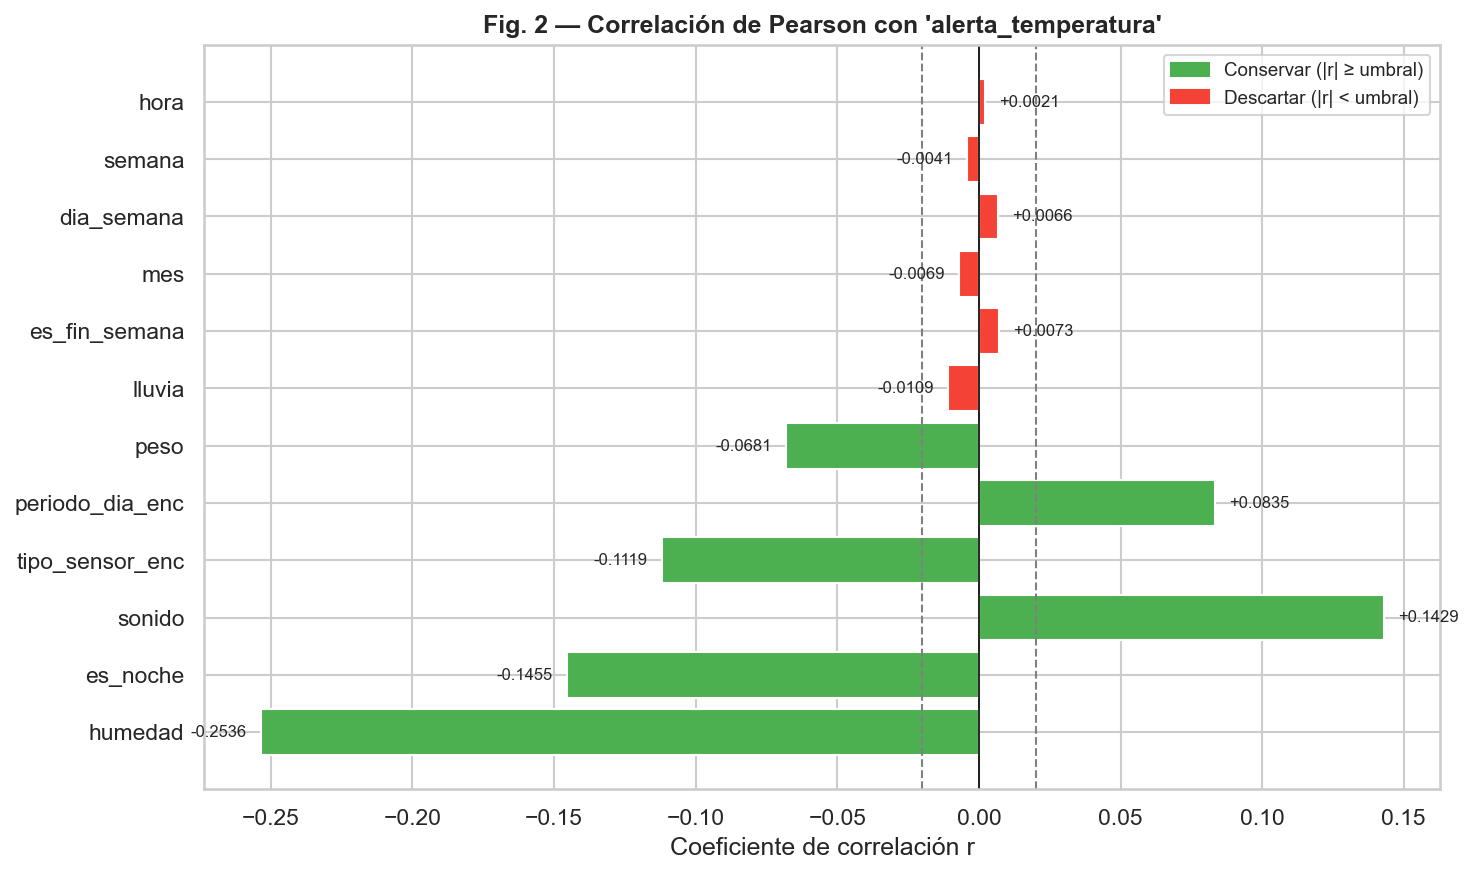
\includegraphics[width=0.9\textwidth]{figures/fig2_pearson_target.png}
  \caption{Coeficiente de Pearson de cada feature con \texttt{alerta\_temperatura}.
           Verde = conservar ($|r| \geq 0.02$).}
\end{figure}

\clearpage

\subsection{M\'etodo 2 --- Umbral de Varianza}

Se descartaron features cuasi-constantes con varianza inferior a 0.01. Ninguna feature
fue eliminada por este criterio, confirmando que todas tienen dispersi\'on suficiente
para aportar informaci\'on al modelo.

\begin{figure}[h!]
  \centering
  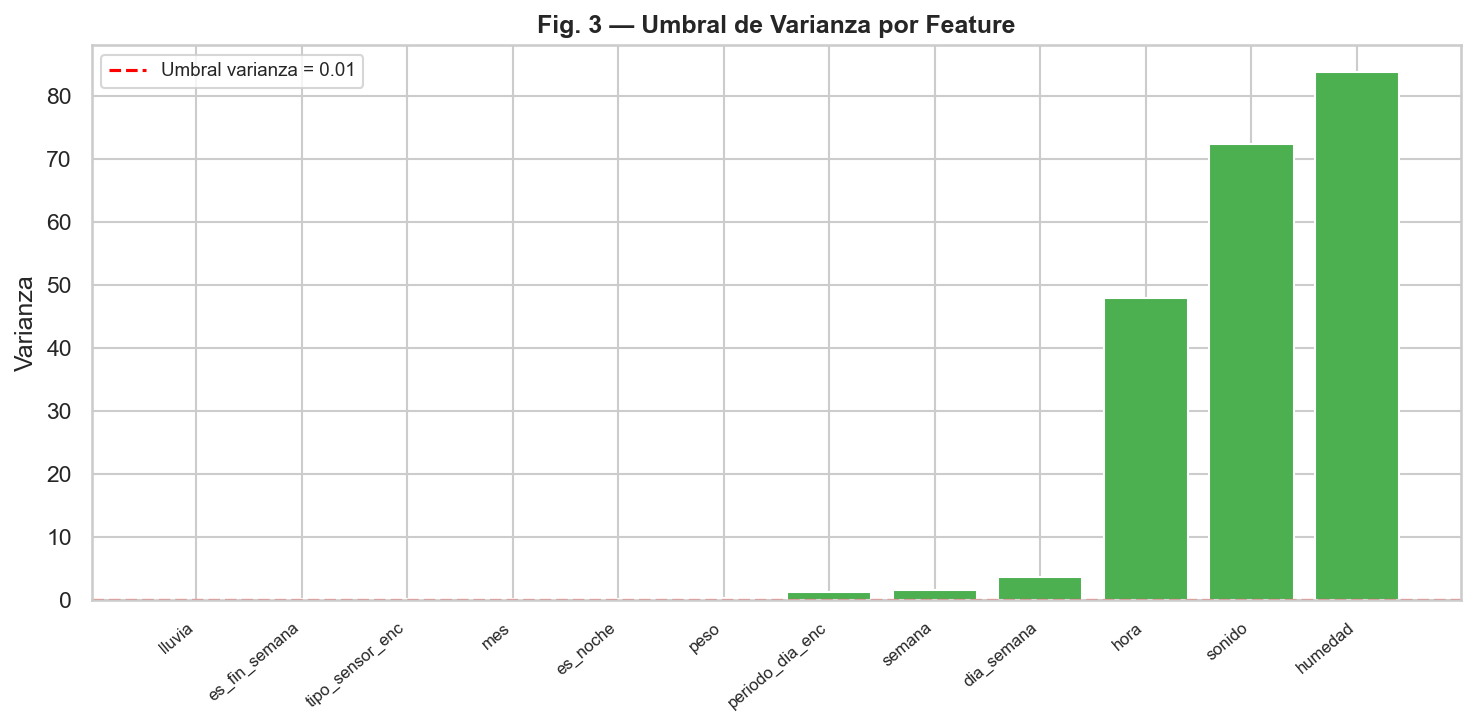
\includegraphics[width=0.9\textwidth]{figures/fig3_varianza.png}
  \caption{Varianza de cada feature. La l\'inea roja marca el umbral de 0.01.}
\end{figure}

\subsection{M\'etodo 3 --- Test Chi-Cuadrado ($\chi^2$)}

El test $\chi^2$ eval\'ua si existe una asociaci\'on estad\'isticamente significativa
entre cada variable discreta o categ\'orica y el target ($H_0$: independencia).
Se rechaza $H_0$ cuando $p < \alpha = 0.05$.

\begin{figure}[h!]
  \centering
  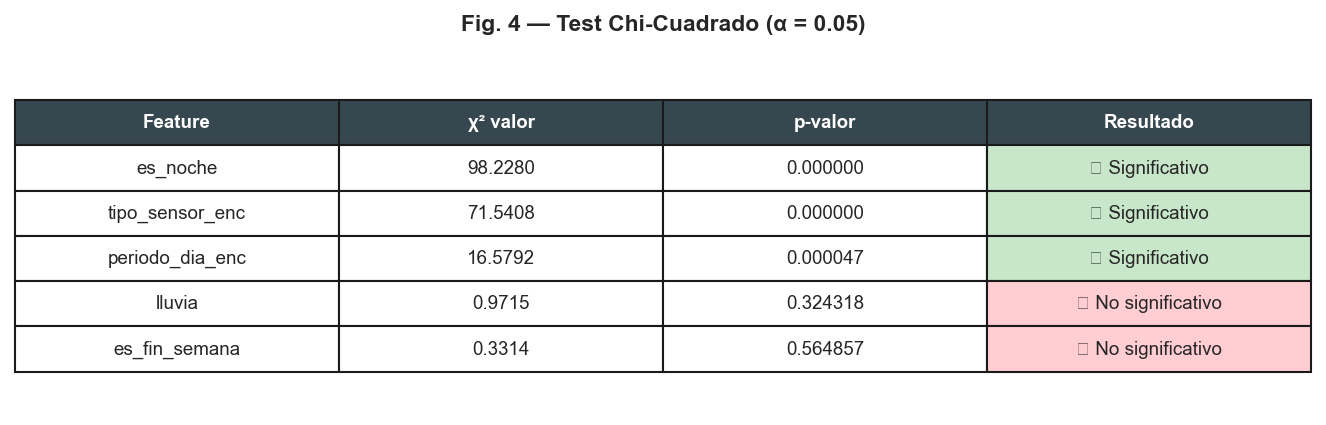
\includegraphics[width=0.85\textwidth]{figures/fig4_chi2_pvalues.png}
  \caption{Resultados del test $\chi^2$. Celdas verdes ($p < 0.05$) indican
           asociaci\'on significativa con el target.}
\end{figure}

\textbf{Descartadas:} \texttt{lluvia} ($p = 0.324$) y \texttt{es\_fin\_semana}
($p = 0.565$). La lluvia no presenta asociaci\'on significativa con alertas de temperatura
porque los eventos de lluvia son independientes del ciclo t\'ermico diario de la colmena.

\subsection{M\'etodo 4 --- Importancia con Random Forest (150 \'arboles)}

Se entren\'o un clasificador Random Forest con 150 \'arboles sobre las features
supervivientes. Las features con importancia Gini inferior a 0.02 se descartaron.

\begin{figure}[h!]
  \centering
  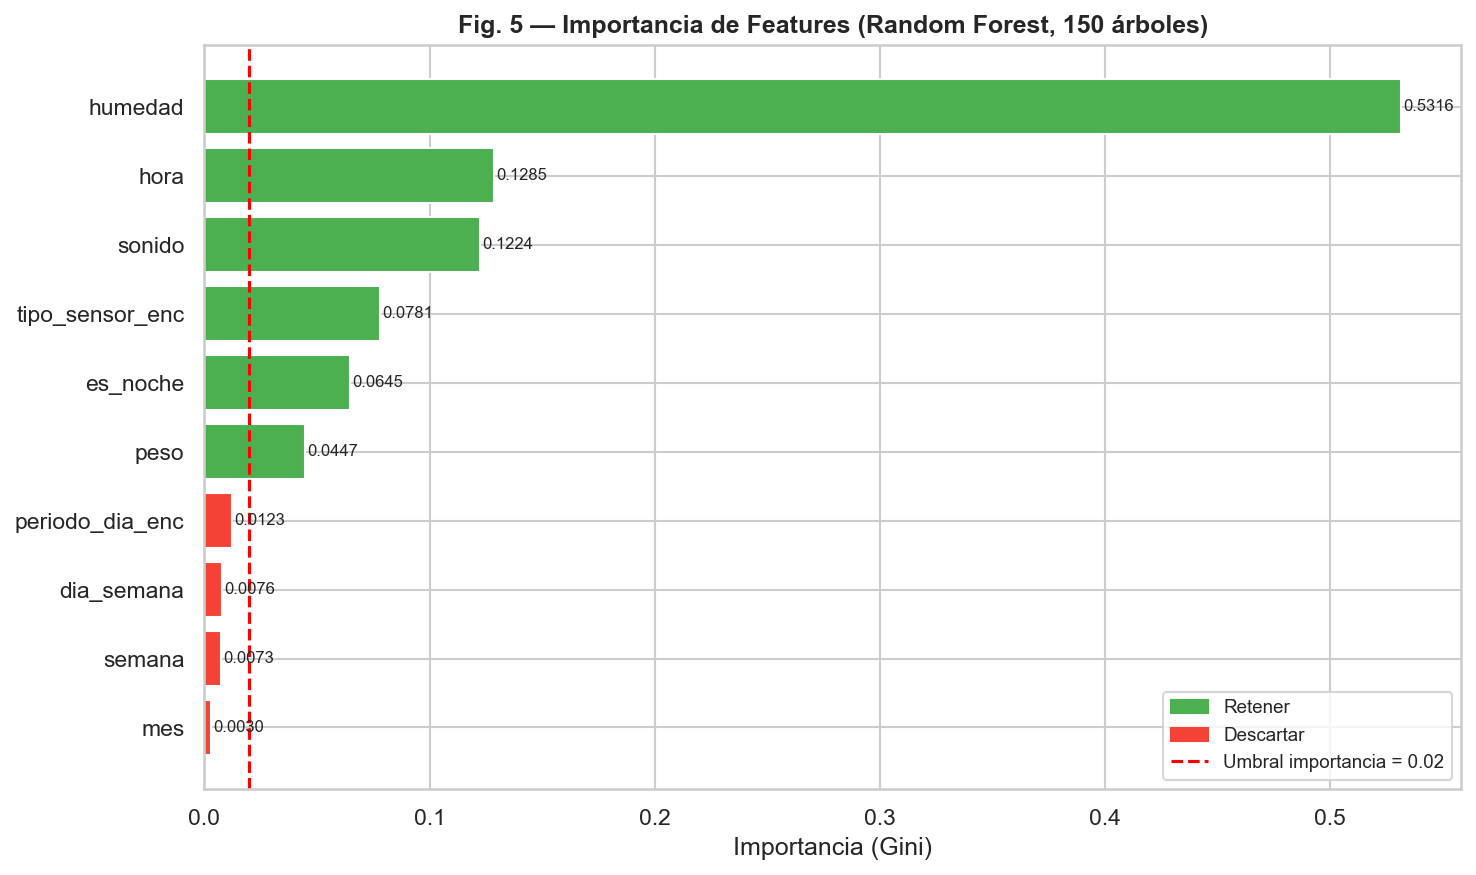
\includegraphics[width=0.9\textwidth]{figures/fig5_rf_importance.png}
  \caption{Importancia Gini por feature. Verde = retenida ($\geq 0.02$),
           rojo = descartada.}
\end{figure}

\clearpage

\subsection{Resumen de Selecci\'on}

\begin{table}[h!]
  \centering
  \caption{Features finales seleccionadas y su justificaci\'on}
  \rowcolors{2}{grisCelda}{white}
  \begin{tabularx}{\textwidth}{lrX}
    \toprule
    \textbf{Feature} & \textbf{Import. RF} & \textbf{Justificaci\'on} \\
    \midrule
    \texttt{humedad}           & 0.5316 & Correlaci\'on inversa fuerte con temperatura ($r \approx -0.8$) \\
    \texttt{hora}              & 0.1285 & La temperatura sigue un ciclo coseno diario con m\'aximo a media tarde \\
    \texttt{sonido}            & 0.1224 & Las abejas \textit{fanners} incrementan la actividad sonora bajo estr\'es t\'ermico \\
    \texttt{tipo\_sensor\_enc} & 0.0781 & Los sensores Multisensor operan en colmenas con distintos microclimas \\
    \texttt{es\_noche}         & 0.0645 & Proxy binario del ciclo d\'ia/noche; temperatura siempre inferior de noche \\
    \texttt{peso}              & 0.0447 & El enjambre por calor puede producir p\'erdida de peso detectable \\
    \bottomrule
  \end{tabularx}
\end{table}

\begin{table}[h!]
  \centering
  \caption{Resumen de reducci\'on dimensional por m\'etodo}
  \rowcolors{2}{grisCelda}{white}
  \begin{tabular}{lr}
    \toprule
    \textbf{M\'etrica} & \textbf{Valor} \\
    \midrule
    Features candidatas iniciales         & 12 \\
    Descartadas por Pearson ($|r|<0.02$)  & 0  \\
    Descartadas por varianza ($<0.01$)    & 0  \\
    Descartadas por Chi-cuadrado ($p\geq0.05$) & 2 \\
    Descartadas por Random Forest ($<0.02$) & 4 \\
    \textbf{Features conservadas}         & \textbf{6} \\
    \textbf{Reducci\'on dimensional}      & \textbf{50\%} \\
    \bottomrule
  \end{tabular}
\end{table}

\subsection{Dataset Final Optimizado}

El archivo \texttt{data/clean/dataset\_final\_features.csv} contiene 8\,573 filas
$\times$ 7 columnas (\texttt{humedad}, \texttt{hora}, \texttt{sonido},
\texttt{tipo\_sensor\_enc}, \texttt{es\_noche}, \texttt{peso},
\texttt{alerta\_temperatura}) y est\'a listo para ser utilizado directamente en el
entrenamiento de modelos de clasificaci\'on (XGBoost, Random Forest, LSTM).
